\documentclass[12pt]{article}

\usepackage{graphicx}
\usepackage{amsmath}
\usepackage{amssymb}
\usepackage{natbib}
\usepackage{amsfonts}
\usepackage{multicol}
\usepackage{float}
\usepackage{oldgerm}
\usepackage{bm}
\usepackage{mathtools}
\usepackage{wrapfig}
\usepackage{fancyhdr}
\usepackage[export]{adjustbox}
\usepackage{xcolor}
\usepackage[shortlabels]{enumitem}

\pagestyle{empty}

\setlength{\headsep}{0.5cm}
\setlength{\oddsidemargin}{-0.5cm}
\setlength{\textwidth}{16.5cm}
\setlength{\textheight}{24cm}
\voffset = -2cm


\pagestyle{fancy}
\fancyhf{}
\rfoot{
\includegraphics[width=1.0in]{cnm.png}}
\lfoot{Homework 10}
\setlength\parindent{0pt}
\begin{document}

\begin{center}
\hfil
{\large\bf {ENGR 2910-101: Circuit Analysis}}
\hfill Instructor: Brian Rashap\\
Homework 10: 04/10/23 \hfill Due: 04/17/23\\
\hrulefill\\
\end{center}

{\bf Question 1} [10] % P9_05

A sinusoidal voltage is zero at $t = -\frac{2 \pi}{3} ms$ and increasing at a rate of $80000 \frac{V}{s}$. The maximum amplitude of the voltage is 80V.

\begin{enumerate}[(a)]
\item What is the frequency of v in radians per second?
\item What is the expression for $v(t)$?
\end{enumerate}

{\bf Question 2} [10] % P9_14

A $50 kHz$ sinusoidal voltage has zero phase angle and a maximum amplitude of $10mV$. When this voltage is applied across the terminals of a capacitor, the resulting stead-state current has a maximum amplitude of $628.32 \mu A$.

\begin{enumerate}[(a)]
\item What is the frequency of the current in radians per second?
\item What is the phase angle of the current?
\item What is the capacitive reactance of the capacitor?
\item What is the capacitance of the capacitor?
\item What is the impedance of the capacitor?
\end{enumerate}

{\bf Question 3} [10] % P9_27

For the circuit shown below:

\begin{figure}[h!]
\begin{center}
 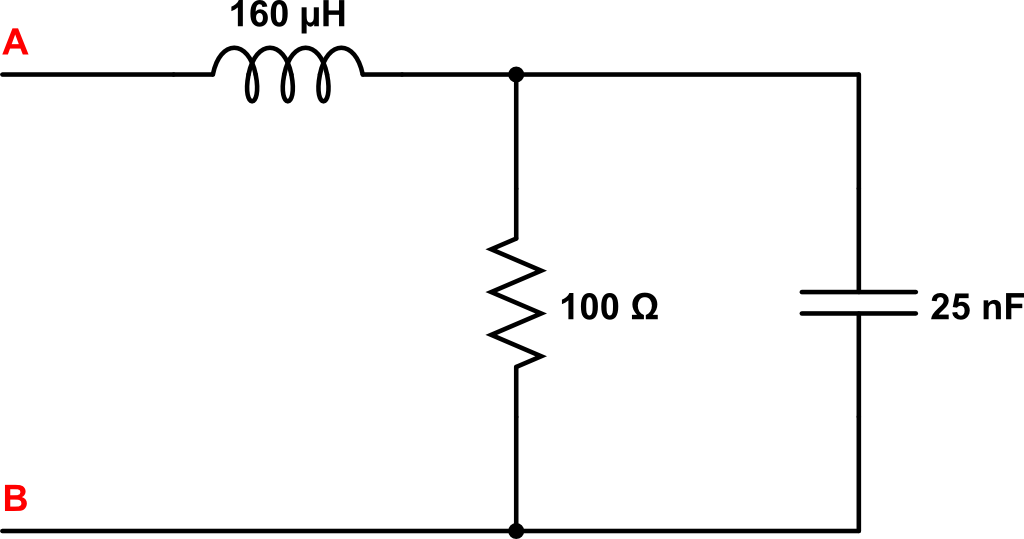
\includegraphics[scale=0.4]{fig9_27.png}
\end{center}
\end{figure}

\begin{enumerate}[(a)]
\item Find the frequency (in radians per second) at which the impedance $Z_{ab}$ is purely resistive.
\item Find the value for $Z_{ab}$ at the frequency found in (a).
\end{enumerate}

\newpage


{\bf Question 4 [10]} % P9_44

Use source transformation to find the Norton equivalent circuit with respect to the terminals a and b for the below circuit when $I_s = 4 \angle 0^{\circ} A$, $L_1 = j 60 \Omega$, and $C_1 = -j 100 \Omega$:

\begin{figure}[h!]
\begin{center}
 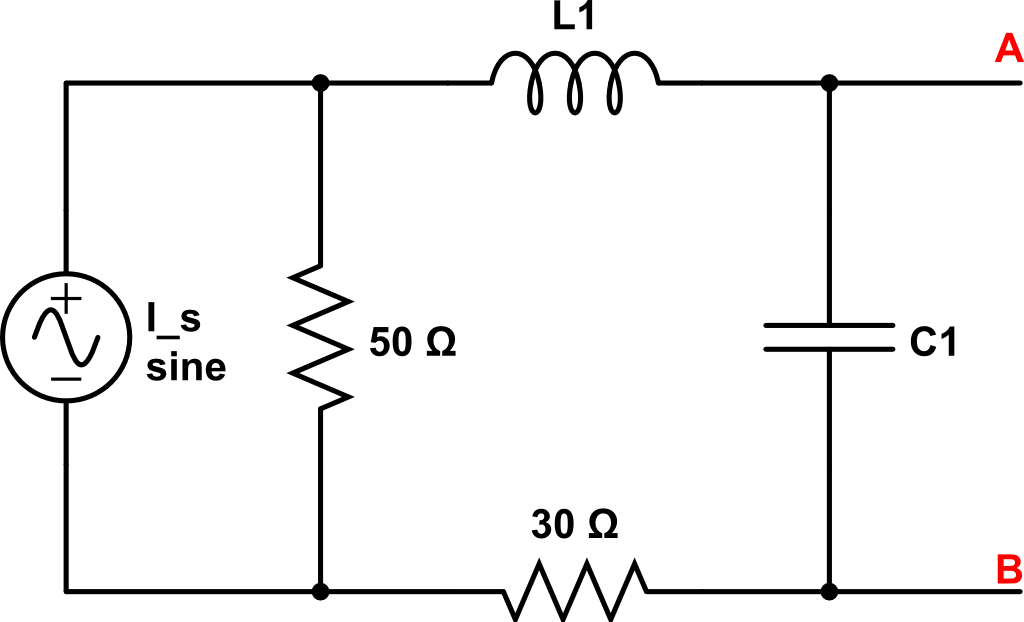
\includegraphics[scale=0.4]{fig9_44.png}
\end{center}
\end{figure}

{\bf Question 5 [10]} % P9_54

Us the node-voltage method to find the steady-state expression for $v_0(t)$ in the circuit below if
\begin{equation}
v_{g1} = 25 \sin{(400t + 143.15^{\circ})} V
\end{equation}

\begin{equation}
v_{g2} = 18.03 \cos{(400t + 33.69^{\circ})} V
\end{equation}



\begin{figure}[h!]
\begin{center}
 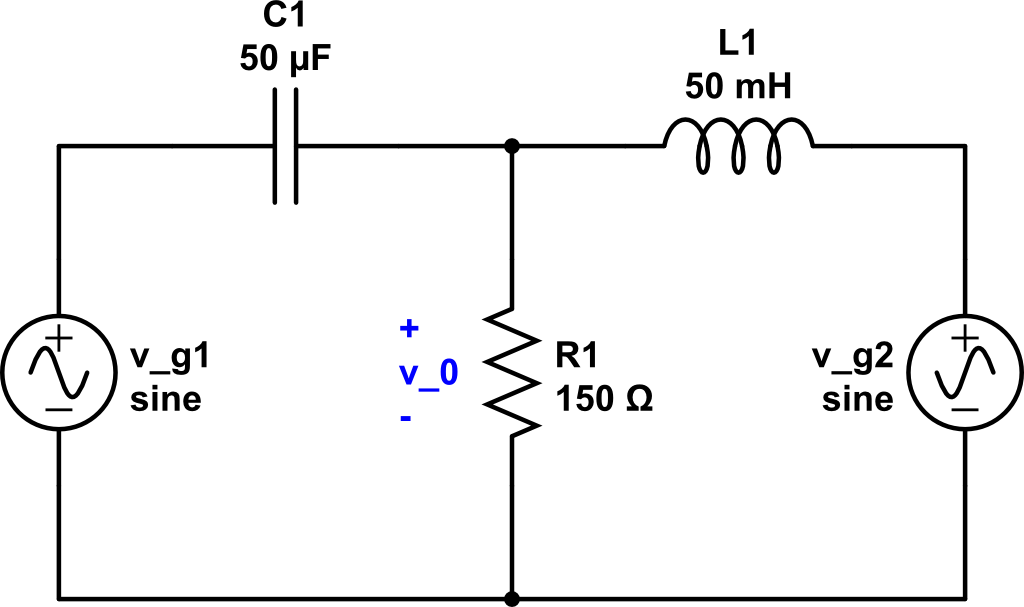
\includegraphics[scale=0.4]{fig9_54.png}
\end{center}
\end{figure}



\end{document}
